\section{Обзор литературы}

\subsection{Нелинейные хромофоры и их применение}

Нелинейные оптические среды~--- это такие среды, в которых вектор поляризации зависит от внешнего электрического поля нелинейно:

\begin{equation}
    \mathbf{P} = \chi^{(1)}\cdot\mathbf{E} + \chi^{(2)}\cdot\mathbf{E}^2 + \ldots
\end{equation}

Такое свойство этих сред позволяет проявляться нелинейными оптическим эфектам: генерации кратных гармоник, сложению частот, генерации разностной частоты и другие многфотонные процессы.

Нелинейность второго порядка позволяет генерировать вторую гармонику и управлять интесивностью нелинейных эффектов с помощью внешнего электрического поля~(эффект Поккельса). Она требует отсутствия центра симметрии в молекуле; на практике это достигается использованием асимметричного донорно-акцепторного хромофора. Второй нелинейный коэффициент образца $\chi^{(2)}$ зависит от молекулярной восприимчивости $\beta$ следующим образом:

\begin{equation}
    \chi^{(2)} = N \beta\ \langle\cos^3\theta\rangle g(\omega),
    \label{eqn:2_nonlinear_coefficient}
\end{equation}

\noindent а основной элемент тензора электрооптического эффекта Поккельса $r_{33}$ выражается как:

\begin{equation}
    r_{33} = \frac{-2\chi^{(2)}}{\eta^4}.
\end{equation}

Таким образом, для максимизации нелинейных свойств хромофоров согласно уравнению~\ref{eqn:2_nonlinear_coefficient} необходимо увеличивать как молекулярную восприимчивость $\beta$, которая зависит от структуры хромофора, так и произведение $N\langle \cos^3\theta\rangle$, которое зависит от расположения молекул хромофора в матрице и межмолекулярного взаимодействия~\cite{Dalton2010a}.

\subsection{Сопряженные донорно-акцепторные (\ac{pushpull}) хромофоры}

Споряженные донорно-акцепторные хромофоры представляют большой интерес из-за их электрооптических свойств: система сопряженных двойных связей позволяет образовать низколежащую \ac{lumo} и реализовать внутримолекулярный перенос заряда. Они применяются в таких областях, как органическая электроника, электрооптика, фотовольтаика~\cite{Bures2014a}.

\begin{figure}
    \centering
    
\includegraphics{sections/literature/img/D-p-A_chromophores.eps}
    \caption{Общая структура \emph{push-pull} хромофоров}
    \label{fig:D-p-A_chromophores}
\end{figure}

\subsection{Донорные блоки}

\subsection{Акцепторные блоки}

\begin{figure}
    \centering
    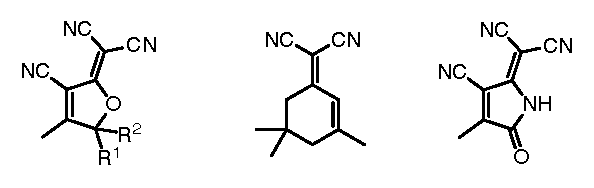
\includegraphics{sections/literature/img/acceptors.eps}
    \caption{Различные акцепторы~\cite{Dalton2010a}}
    \label{fig:acceptors}
\end{figure}

\subsection{Влияние дендроидного заместителя}

\subsection{Подходы к синтезу триарилпиразолинов}
2-пиразолины~(\ref{fig:pyrazoline_structure}) были впервые синтезированы в 19 веке Фишером и Кнёвенагелем реакцией $\alpha,\beta-$ненасыщенных альдегидов и кетонов с фенилгидразином при кипячении в уксусной кислоте.

В недавнее время были предприняты попытки проводить реакцию в более экологичных условиях, используя в качестве циклизующего агента вольфрамсерную кислоту~\cite{Rahmatzadeh2015} и целлюлозосульфоновую кислоту~\cite{Daneshfar2015}. Также в качестве экологически чистых методов исследовались синтез в водных растворах~\cite{Markovic2015}, механохимический синтез~\cite{Zangade2013}, микроволновый синтез~\cite{Adhikari2012} и ультразвуковой синтез~\cite{Shelke2012}.

\begin{figure}
    \centering
    \includegraphics{sections/literature/img/pyrazoline_structure.eps}
    \caption{Структура и нумерация атомов 2-пиразолина}
    \label{fig:pyrazoline_structure}
\end{figure}

Основным способом синтеза 1,3,5-триарилпиразолинов является реакция конденсации халконов с арилгидразинами. Установлено, что обычно первым вступает в реакцию вторичный атом азота, реагируя с двойной связью халкона. Далее второй атом азота реагирует с карбонильной группой, замыкая пиразолиновый цикл. Этот подход является достаточно общим, как было показано в работе~\cite{Powers1998}, где таким способом была получена библиотека из \num{7680} соединений с различными заместителями во всех трех ароматических ядрах.

\begin{scheme}
    \centering
    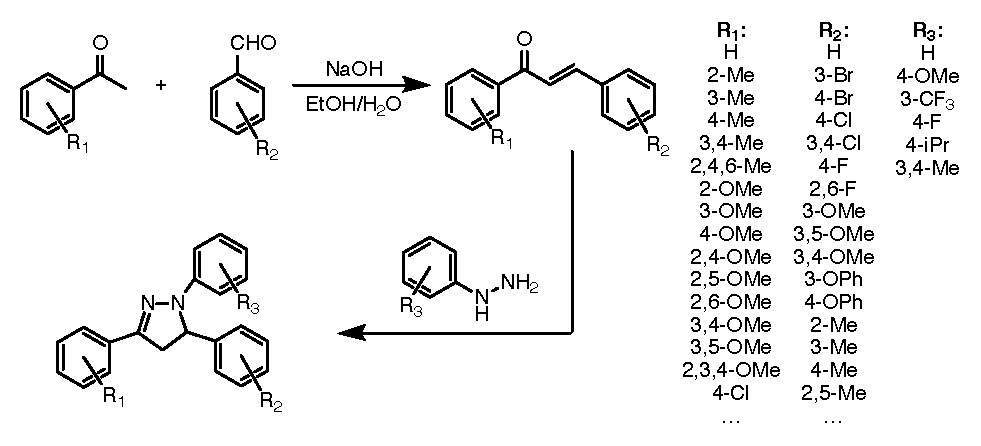
\includegraphics{sections/literature/img/pyrazolines_common.eps}
    \caption{Cинтез триарилпиразолинов с использованием халконов}
\end{scheme}

Получение полифторованных триарилпиразолинов несет в себе больше сложностей: в случае разных заместителей халкона часто не удается подобрать условия реакции таким образом, чтобы получать селективно один региоизомер~--- образуется смесь продуктов с разными заместителями в положениях 3 и 5.

\begin{scheme}
    \centering
    \includegraphics{sections/literature/img/polyflouro_isomers.eps}
    \caption{Образование двух региоизомеров 2-пиразолина}
    \label{sch:polyflouro_isomers}
\end{scheme}

Второй способ синтеза пиразолинов использует [3 + 2] циклоприсоединение илидов азометиновых иминов к алкинам. [3 + 2] циклоприсоединение 1,3-диполей к диполярофилам является удобным способом получения пятичленных циклов. Наиболее известным примером таких реакций является присоединение азидов к алкинам. Считается, что [3 + 2] циклоприсоединения идет по согласованному механизму. Использование комплексов металлов с хиральными лигандами в качестве катализаторов позволяет селективно получать энантиомерно чистые пиразолины. Циклоприсоединение илидов азометиновых иминов к алкенам дает полностью насыщенные аналоги пиразолинов~--- пиразолидины~\cite{Groselj2018}. \todo[inline]{Какой-то несогласованный абзац}

\begin{scheme}
    \centering
    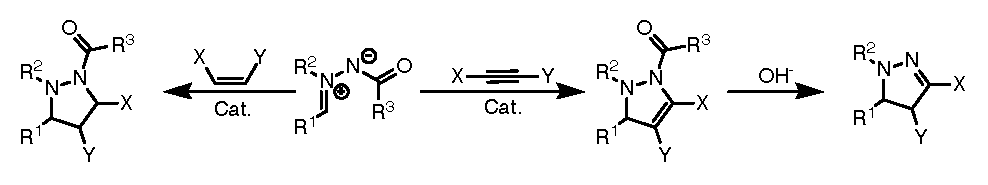
\includegraphics{sections/literature/img/pyrazolines_cycloaddition.eps}
    \caption{Синтез триарилпиразолинов с использовнием [3 + 2] циклоприсоединения}
\end{scheme}


Азометиновые имиды можно представить в виде четырех резонансных структур~(\ref{fig:azomethine_resonance})~--- двух иминных и двух диазониевых. Чаще всего их изображают с зарядами, локализованными на атомах азота, такое распределение зарядов соотносится с квантовомеханическими расчетами~\cite{Groselj2018}.

\begin{figure}
    \centering
    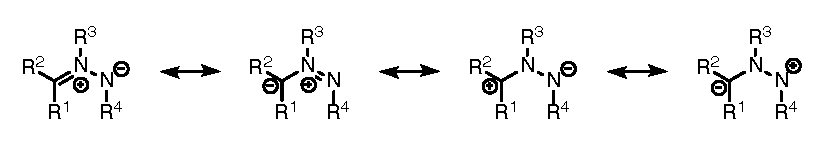
\includegraphics{sections/literature/img/azomethine_resonance.eps}
    \caption{Резонансные структуры илидов азометиновых иминов}\label{fig:azomethine_resonance}
\end{figure}

Существует несколько способов получения илидов азометиновых иминов в основном \ac{insitu}, включающие генерацию из гидразонов с последующим [3 + 2] циклоприсоединением, генерацию из енгидразинов, взаимодействие 1,2-дизамещенных гидразинов с карбенами, взаимодействие азосоединений с диазоалканами, окисление N,N,N'-тризамещенных гидразинов, 1,4-силаторпный сдвиг в $\alpha$-силилнитрозаминах и $\alpha$-силилнитрозамидах и метатезис 1,2-диарилдиазен-1-оксидов~\cite{Padwa2005}.

\begin{scheme}
    \centering
    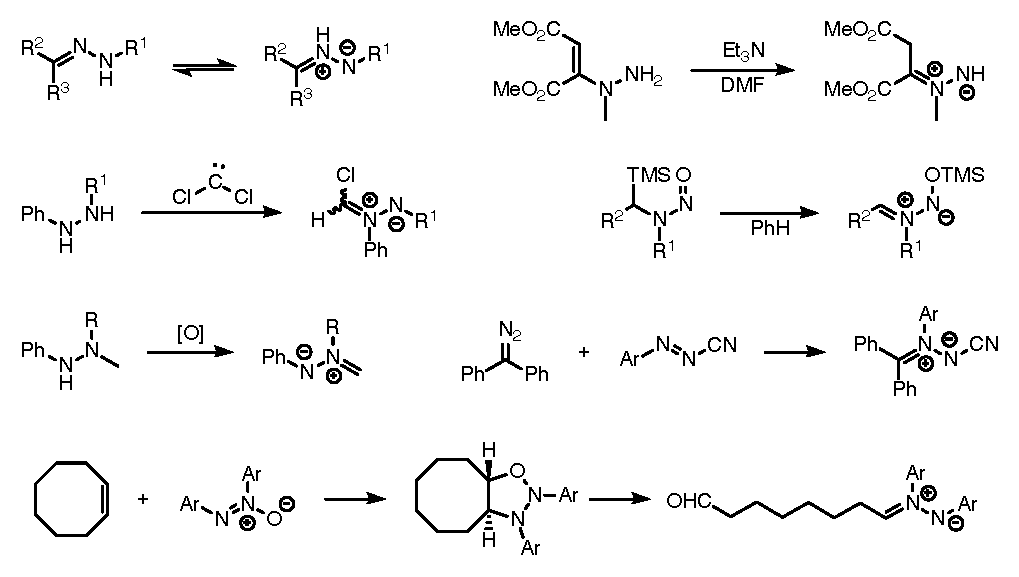
\includegraphics{sections/literature/img/azomethine_generation.eps}
    \caption{Различные способы получения илидов азометиновых имидов}
\end{scheme}

Синтез пиразолинов, исходя из ациклических илидов азометиновых иминов, получаемых \ac{insitu}, был подробно изучен в работе~\cite{Hashimoto2013}. В этой работе было синтезировано более \num{18} пиразолинов и проведена оптимизация условий реакции: было изучено влияние различных солей \ce{Cu(I)}, заместителей лигандов и субстратов.

\begin{scheme}
    \centering
    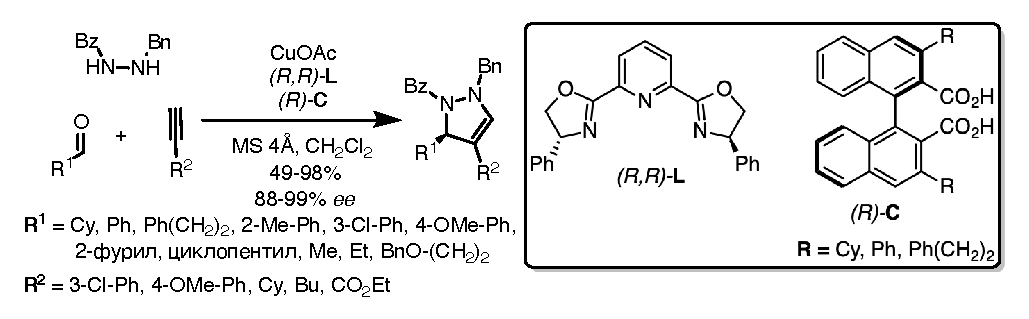
\includegraphics{sections/literature/img/cycloaddition_example.eps}
    \caption{Энантиоселективный синттез пиразолинов с использованием [3 + 2] циклоприсоединения~\cite{Hashimoto2013}}
\end{scheme}
